% ==============================================================================
% Supplementary Figure 6: LaTeX Code & Caption for Nature Communications
% Location: 04_Figure_Generation/Supplementary_Figure_06/Supplementary_Figure_6_Caption.tex
% ==============================================================================

\begin{figure}[p]
\centering
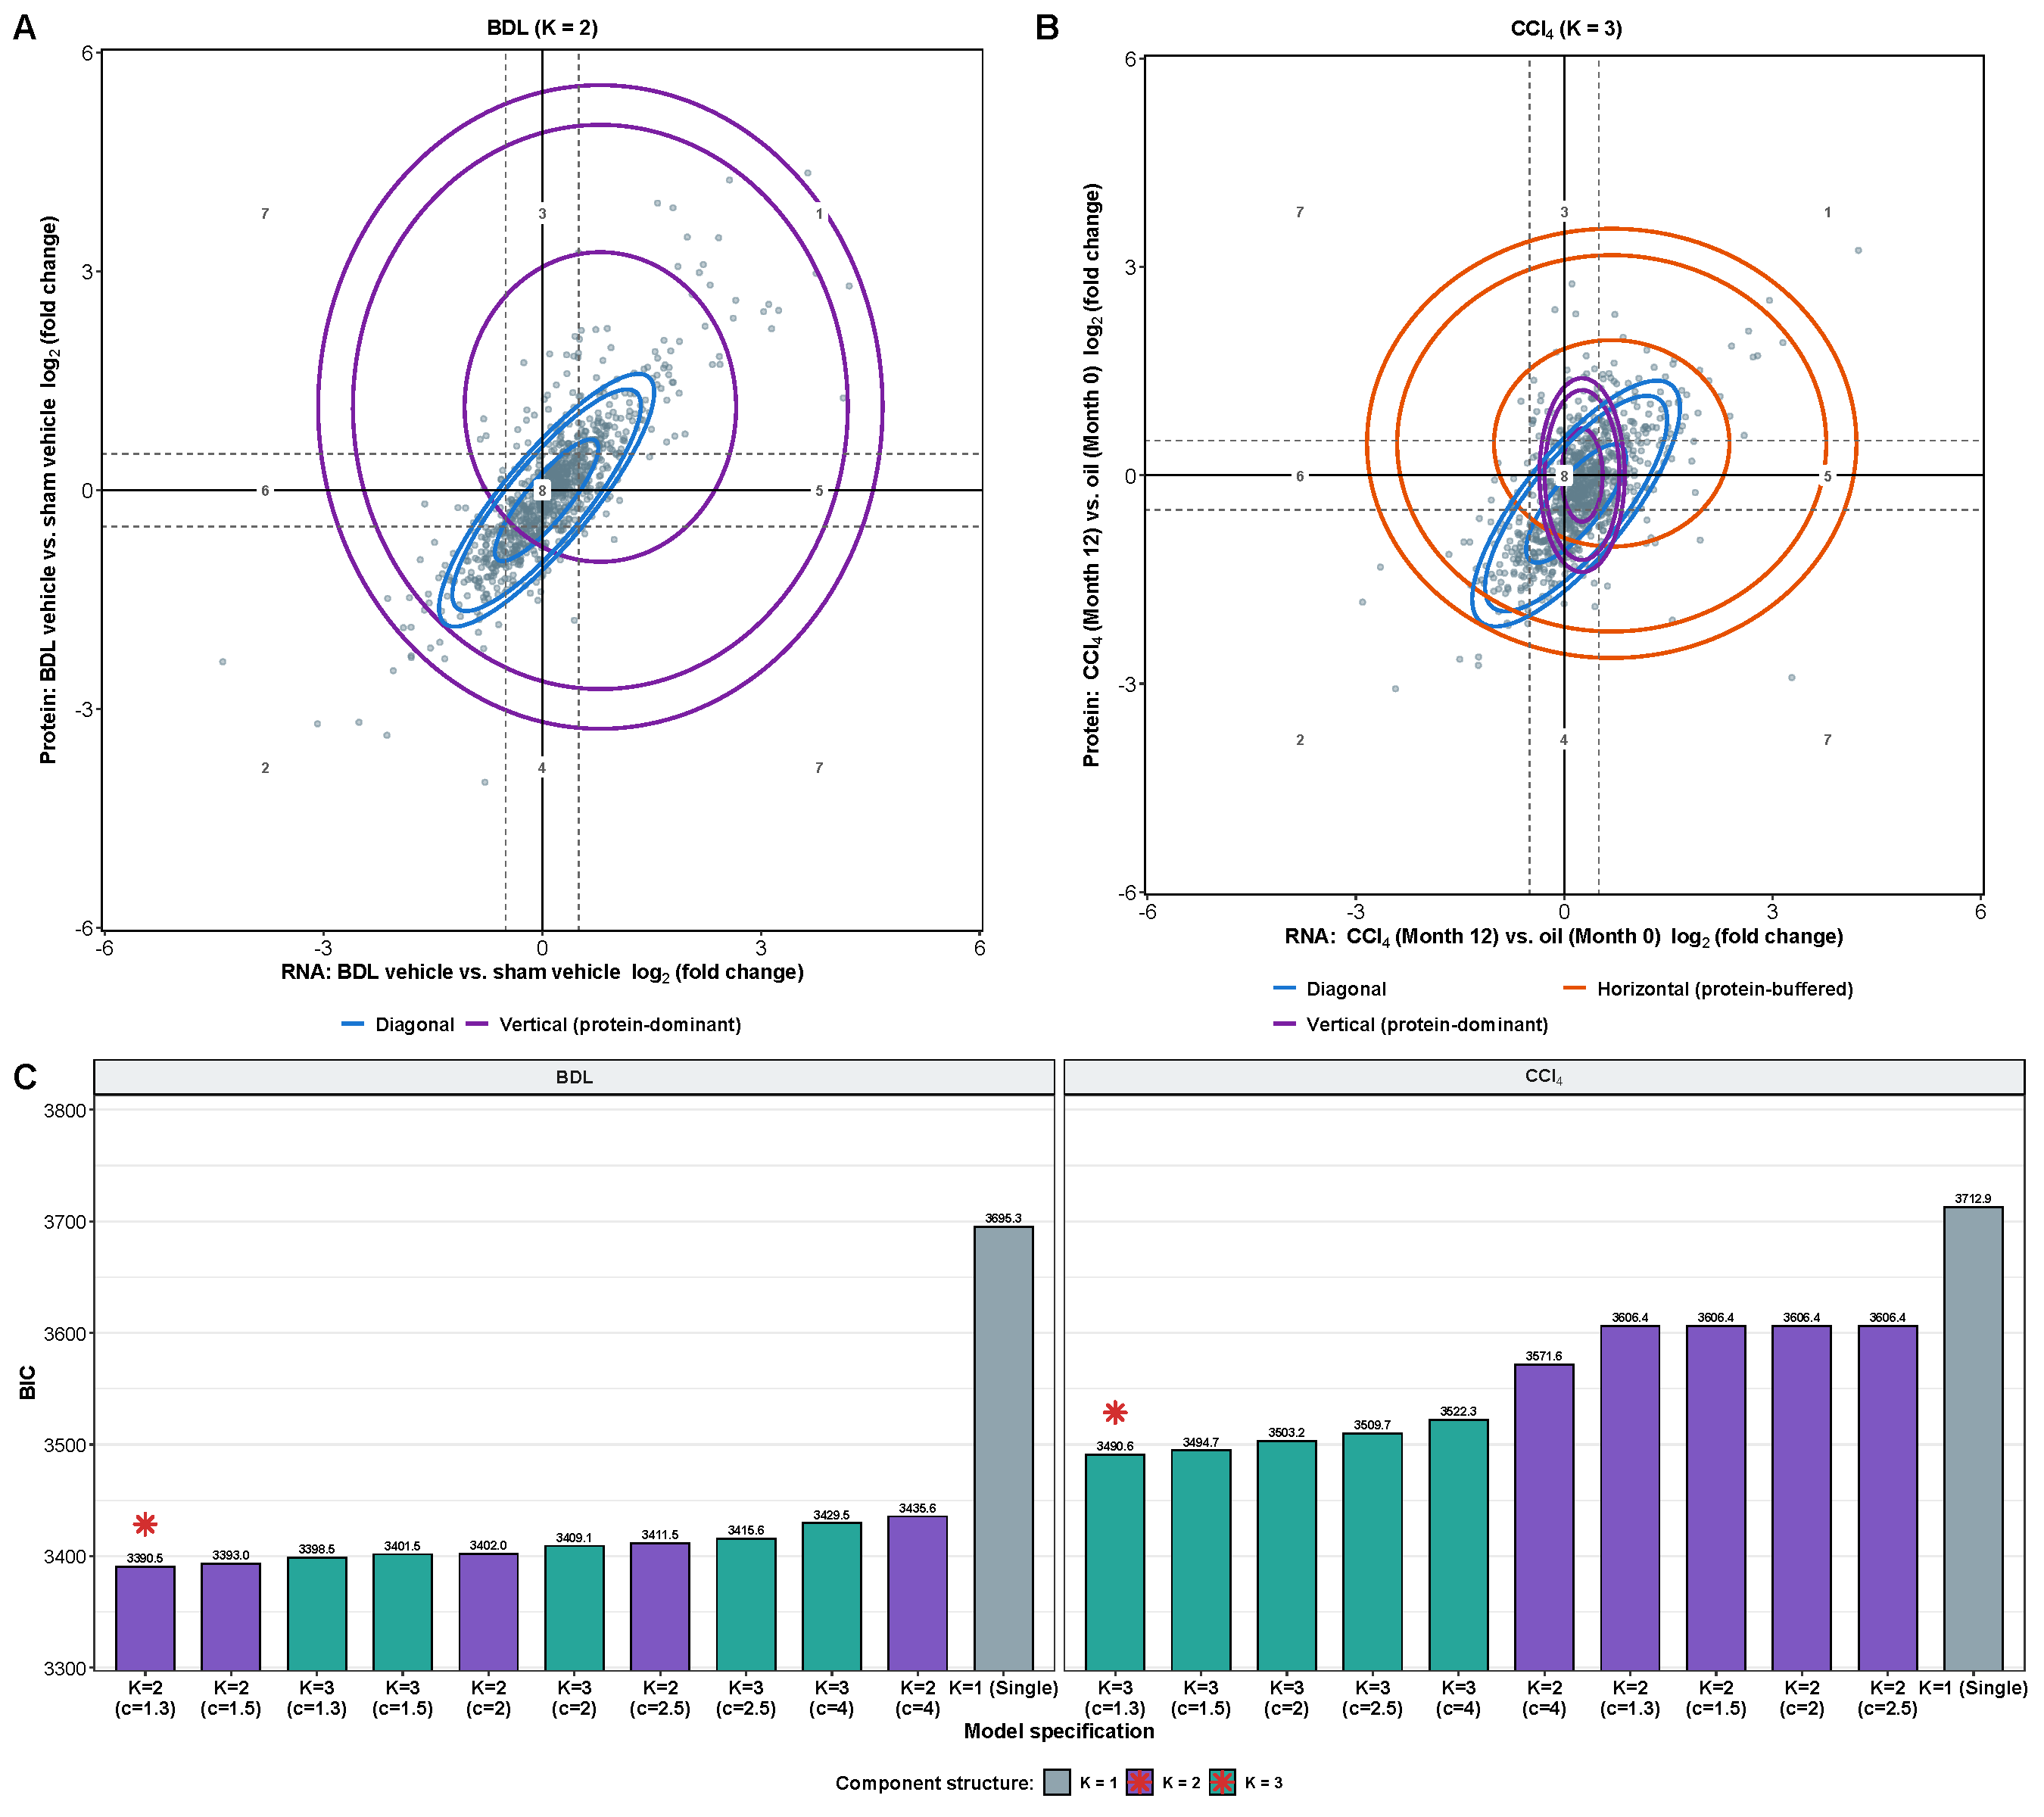
\includegraphics[width=\textwidth]{Supplementary_Figure_6.pdf}
\caption{\textbf{Constrained bivariate Gaussian mixture modeling and model selection of mRNA--protein fold change distributions.} 
\textbf{A,} Bivariate distribution of mRNA and protein $\log_2$ fold changes under cholestatic liver injury (BDL dataset, $N = 943$ matched gene--protein pairs). Blue and purple solid contours depict the 50\%, 90\%, and 95\% concentration ellipses of the winning two-component constrained Gaussian mixture model ($K = 2$, minimum elongation factor $c = 1.3$). The dominant Component~1 (blue, 90.9\% mixing proportion) captures canonical synchronous coupling ($\rho_1 \in [0.70, 0.90]$), while Component~2 (purple, 9.1\%) captures vertically oriented, protein-dominant decoupling ($\sigma_{y2}^2 \ge 1.3\,\sigma_{x2}^2$). Dashed grey lines denote the empirical $\pm 0.5\,\log_2\text{FC}$ boundaries defining the DiPa quadrants (numbered 1--8). 
\textbf{B,} Bivariate distribution of mRNA and protein $\log_2$ fold changes under toxic liver injury ($\text{CCl}_4$ dataset, Month 12 vs Month 0, $N = 943$ matched gene--protein pairs). Solid contours represent the 50\%, 90\%, and 95\% concentration ellipses of the favored three-component model ($K = 3$, $c = 1.3$), resolving diagonal coupling (Component~1, blue, 61.6\%), vertical protein-dominant decoupling (Component~2, purple, 30.2\%), and horizontal transcriptomic buffering (Component~3, orange, 8.2\%; $\sigma_{x3}^2 \ge 1.3\,\sigma_{y3}^2$). 
\textbf{C,} Information-theoretic model selection across component complexities ($K = 1, 2, 3$) and elongation constraints ($c \in \{1.3, 1.5, 2.0, 2.5, 4.0\}$). Bars display the absolute Bayesian Information Criterion (BIC, where lower values indicate superior parsimony and goodness-of-fit), sorted in ascending order (from lowest to highest BIC) for each cohort. Numbers above each bar indicate the absolute BIC value. Red asterisks denote the overall winning model in each etiology ($K = 2, c = 1.3$ for BDL with $\Delta\mathrm{BIC} = -304.8$ relative to the single-Gaussian null model; $K = 3, c = 1.3$ for $\text{CCl}_4$ with $\Delta\mathrm{BIC} = -222.3$). Source data are provided in Supplementary Table~5.}
\label{fig:suppl_fig_06}
\end{figure}
